
%%% Local Variables:
%%% mode: latex
%%% TeX-master: t
%%% End:

\chapter{引言}
\label{chap:intro}

互联网与云计算的发展,越来越多的应用从本地迁移到云端,并涌现出大量新兴的互联网应用,
承载这些应用的数据中心成为了如同电力系统一样的社会基础设施。
与此同时,现代数据中心正在面临着权衡资源利用率与应用服务质量的挑战:
从应用开发者角度,服务质量是第一位的,因为它直接关系到用户体验与其收益,
由于互联网应用负载的波动性,开发人员通常会为自己的应用过量分配资源以满足峰值时的负载需求,
这造成了非常低的服务器利用率,通常只有6\%-12\%;
而对于数据中心运维人员,资源利用率直接反映其运维成本,虽然将不同应用混合部署到同一台服务器,
充分利用空闲时段的服务器资源可以有效提高数据中心利用率,
但多应用混合部署引入的软硬件资源共享会造成应用间无管理的资源竞争,
使得应用性能出现不可预测的波动,进而影响应用的服务质量。
由上可知,如何权衡数据中心资源利用率与应用服务质量是当前数据中心亟待解决的重要问题。

可以从三个角度解决这一问题:
其一是通过上层软件机制实现干扰容忍,在应用层保障服务质量,
如Google提出的Hedged Requests和Tied Requests方案\cite{dean_tail_2013},
通过向多个副本发送请求,并选择最快返回的结果以达到干扰容忍的目的。%Timecard和D2P
其二是在应用调度层次,通过profile的方式预测应用混合后的干扰情况,
将相互之间干扰较小的应用部署到同一台服务器。
其三是提供一个良好的隔离环境,降低由资源竞争所产生的应用间干扰,
可以在各个层次实现隔离,如操作系统级\cite{cgroup}、Hypervisor级\cite{}、硬件级\cite{}。

其中前两种方案在实施时需要对目标应用具有非常深入的理解:
方案一需要对应用架构与实现细节进行修改,以达到应用层干扰容忍的目的;
方案二虽然无需对应用进行修改,但需要对应用的资源占用以及不同应用之间的干扰状况进行分析,
才能得到最优的调度方案。
当应用数量不多且有条件进行以上所述的分析或修改,通过精细的应用架构设计与调度机制,
可以有效的解决前文所提到的资源利用率与服务质量相冲突的问题。
但在现实数据中心特别是云计算数据中心内,以上假设并不成立。

首先,数据中心内通常会运行大量的应用,如Google的数据\cite{}表明其数据中心在两个月内累计运行超过2000000个应用,
无论是改造这些应用或是对应用之间的干扰行为进行分析都是不可行的。
即使只对部分关键的应用进行改造使其适应干扰环境,云计算环境下的“吵闹的邻居(Noisy Neighbors)”也会使这些努力的结效果大打折扣。

其次,调度方案无法解决短时运行的干扰应用对其它正常应用带来的影响,特别是随着DevOps的兴起,
由于开发调试与线上部署是不断迭代进行的,调试过程中所引入的短时干扰应用数量大大增加,
Google的数据\cite{}发现大量的小于6分钟的应用都是来自于这些调试应用。
当调度器发现干扰并准备采取调度措施时干扰应用可能已经结束,同时新的干扰应用又开始运行,并带来新的干扰。

当前对第三种隔离方案也有很多研究,包括在软件栈各个层次如虚拟化层\cite{}、操作系统内核层\cite{}、网络协议栈\cite{}等的隔离。
由于在软件层次只能做到较粗粒度的资源管理,实现的效果有限;
同时应用的不同特征造成资源竞争点是分布在整个软件栈中,因此只能根据实际场景做针对性的优化;
再次,在如此复杂的软件栈中找到真正的资源竞争点需要大量的时间与精力,这同样不能满足云计算的场景下应用多样与快速部署的需求。
除了软件栈上的共享,混合部署的应用在硬件层次上也存在大量的共享,如CPU末级缓存、内存控制器、I/O等,
另一些研究专注于如何在这些共享硬件上提供隔离功能,典型的工作如末级缓存划分\cite{}和内存控制器划分\cite{},
但这些研究大都只关注于一种类型的资源,而且是针对特定的场景,因此缺少灵活的软件编程接口,不能适用于通用的计算场景。

综上可知,现有的三种方案都不能很好的解决当前云计算数据中心中遇到的资源利用率与服务质量矛盾的问题,
该问题的本质是为应用提供区分化服务,而如何解决目前计算机系统的软硬件资源的无管理共享状态是实现区分化服务的关键。
现有研究在一定程度上能够解决软件层次的共享管理问题,但无管理的硬件共享使得该问题并没有被完全解决。
造成这一现状的原因是目前的计算机体系结构在设计时并没有考虑到多应用共享场景,
其指令集抽象不足以将上层应用需求传递到下层硬件,在不能区分应用需求的前提下很难做到区分化服务。
软件层次已有很多方案可以用于区分不同应用,如操作系统级的进程PID或cgroup,或更细粒度的应用级标签。%\cite{zhangxd:software-defined-storage, timecard, d2p, ...}
硬件层次也需要一种应用需求传递机制,正如“21st Century Computer Architecture”白皮书中所提出的:

\begin{quotation} 
\emph{\textbf{Better Interfaces for High-Level Information.}
Current ISAs fail to provide an efficient means of capturing software-intent or conveying critical high-level information to the hardware.
For example, they have no way of specifying when a program requires energy efficiency, robust security, or a desired Quality of Service (QoS) level.
Instead, current hardware must try to glean some of this information on its own ......
% - such as instruction-level parallelism or repeated branch outcome sequences - at great energy expense. 
\textbf{New, higher-level interfaces are needed to encapsulate and convey programmer and compiler knowledge to the hardware,}
resulting in major efficiency gains and valuable new functionality.}\cite{21st_architecture}
\end{quotation}

因此要实现高效通用数据中心目标,核心是从硬件上改变资源的“无管理共享”现状以实现在体结构上支持应用服务质量保障,在
此基础上实现数据中心资源根据应用动态管理以提高资源利用率。

\begin{figure}[H]
  \centering
  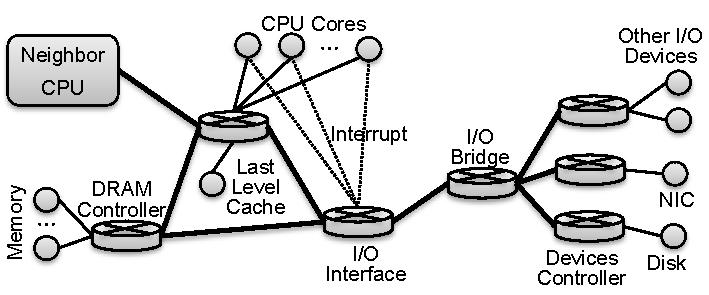
\includegraphics[height=4cm]{intro/computer-as-a-network.pdf}
  \caption[计算机内部本质是一个网络]{
    计算机内部部件之间以数据包(packet)进行通信,比如
    处理器核之间使用基于包的片上网络、
    处理器之间采用基于包的互连协议(如QPI和HT)、
    I/O设备与内存之间则通过PCI-E包进行通信。
    因此,计算机本身即可视为一个网络。}
  \label{fig:computer-as-a-network}
\end{figure}

本文提出了一种新体系结构:资源按需管理可编程的体系结构PARD\cite{pard2015},
使数据中心服务器能够支持区分化服务,通过细粒度的硬件资源管理以及灵活的编程接口,
实现在保障关键应用服务质量的前提下提高服务器资源利用率。
PARD体系结构的核心是基于一个重要的观察:\textbf{计算机内部本质上是一个网络}。
如图\ref{fig:computer-as-a-network}所示,
CPU核、共享缓存、内存控制器、I/O设备等可以被看做是网络节点,它们之间也通过包进行通信;
除了处理请求以外,这些“网络节点”与网络中的路由器/交换机具有相似的请求转发功能。
在网络领域,如何实现端到端的服务质量保障已有大量的研究,并已形成标准。
如IETF(Internet Engineering Task Force, 互联网工程任务组)于1998年提出了区分化服务
(Differentiated Services)\cite{}的概念,
如今区分化服务已经成为应用最广泛的服务质量保障机制之一;
软件定义网络(SDN)的出现,进一步促进了网络领域服务质量保障的发展,其提出的
(1)控制平面与数据平面分离,和(2)集中控制的统一编程接口,
为网络管理带来了极大的灵活性。
本文希望能够将网络领域的区分化服务和软件定义网络的思想应用到计算机内部的网络,
用以解决数据中心当前面临的资源利用率与应用服务质量矛盾。

PARD体系结构的核心设计理念可以归结为以下四点:
\textbf{(1)标签机制},
通过在请求源(如处理器核或具有DMA功能的I/O设备)增加标签寄存器,使用其记录当前正在使用该部件的应用标签,
发出请求时附带该标签,并随着请求在整个计算机内部传播,实现应用区分;
\textbf{(2)可编程控制平面},	%其实是数据平面
为共享硬件资源的控制器增加控制平面,控制平面可根据请求标签查询规则进行区分处理,该规则可通过软件实现可编程;
\textbf{(3)节点内统一资源管理},
节点内所有的控制平台通过控制面网络连接到资源管理模块,提供对控制面的编程接口,实现所有共享资源的统一管理;
\textbf{(4)Trigger=>Action编程方法},
一种基于动作触发的资源管理策略,实现资源实时监控和调整。

本文后续章节将讨论如何在现有体系结构上扩展以实现标签机制;
通用控制平台的设计以及可编程机制的实现,并包括末级缓存控制器和内存控制器中控制平面的具体设计;
基于以上两种机制实现无Hypervisor的全硬件支持虚拟化系统,以及如何实现资源按需分配的区分化服务。
最后在基于模拟器和FPGA的原型系统中验证PARD体系结构的效果,并讨论了原型系统实现过程中的经验与教训。


\section{本文的主要贡献}

本文的论点是:在应用数量众多、需求多样且不断变化的数据中心场景下,计算机体系结构需要重新设计,
为应用提供区分化服务、良好的性能隔离,并具备灵活的资源管理编程接口,实现资源的按需分配,
才能解决数据中心资源利用率与服务质量冲突的问题。

本文的主要贡献包括:

% 可在多个层次(虚拟机、进程、线程、API、...)区分应用,实现了NoHyper功能
第一,提出“标签化地址空间(Labeled Address Space)”概念 。
使用统一标签区分不同应用,并为计算机系统内所有请求标识应用标签,
硬件不再需要通过猜测的方式区分应用,而是通过标签机制打破目前体系结构中软硬件之间的语言鸿沟,
使得共享的硬件资源能够区分来自不同应用的请求并进行区分处理。
可在不同层次实现应用区分,如虚拟机、进程、线程或使用API标识的数据/代码段,以实现不同粒度的区分化服务。
以虚拟机粒度为例,通过标签机制以及共享硬件资源内部基于标签的划分机制,
可将一台计算机划分为多台独立的逻辑域(Logical Domain),在每个逻辑域内独立运行操作系统,
实现NoHyper\cite{nohype2012}的功能。

% 表+Trigger/Action <=> 处理器方案
第二,提出共享硬件资源管理方法,为硬件资源共享方法提供配置、监控、反馈功能,实现毫秒(ms)级的性能反馈。
实时的监控与反馈是实现细粒度资源管理的重要前提,软件监控方案无法满足实时性的需求,
本文提出将资源监控与硬件资源结合,在硬件上直接实现监控与反馈,提出使用通用的“控制平面”实现硬件资源的配置与监控,
具体包含基于表的简单控制与基于处理器的复杂控制两种实现。为计算机系统实现可管理提供支持。

第三,提出节点内硬件共享资源的协同管理。通过使用控制面网络将所有的控制平面连接到集中式的资源管理模块,
对硬件共享资源进行统一管理。

以上三点贡献已在PARD的模拟器及FPGA原型系统中实现。
模拟器原型是基于gem5实现的全系统时钟精确模拟器,增加或修改了大约XXX行C++代码,该模拟器以在LGPL协议下开源。
FPGA原型系统基于MicroBlaze系统在Xilinx VC709开发板实现并完成验证,系统运行在133MHz主频,包含4个处理器核。
两个原型系统可以做为后续相关研究的参考平台。


\section{论文的组织}

本文共分八章,
第二章介绍数据中心面临的资源利用率与服务质量冲突问题的挑战,然后讨论现有数据中心技术的局限性,
并介绍解决该问题的现有研究。

第三章介绍PARD体系结构与关键特性。通过管理员视角说明该系统如何工作。

第四章介绍标签化地址空间的原理与实现,
对现有体系结构的服务质量支持进行评估,包括软件(cgroup, hyperviso)和硬件两个层次。
介绍资源管理可编程体系结构的概念与核心思路,并将其映射到现有体系结构,
讨论其可行性。同时应用资源管理可编程体系结构实现全硬件虚拟化,并讨论其关键技术。

第五章讨论共享资源控制平面设计,与资源管理可编程实现,
硬件支持、Trigger-Action机制,模拟的方式验证PARD的有效性。

第六章介绍资源管理模块与资源协同管理相关的内容,包含节点内与数据中心级协同资源管理。

第七章基于前两章的设计给出本文资源管理可编程体系结构的FPGA原型系统实现,
并对原型系统各部分功能的正确性、性能与开销进行了详细评测。

第八章总结全文并介绍未来可能的研究工作。
